\section{Các Mô hình Sinh Đa phương thức (Multimodal Generative Models)}
\label{sec:multimodal_generative_models}

\subsection{Tổng quan: Hợp nhất các Giác quan Kỹ thuật số}
\label{subsec:multimodal_gen_overview}
Các làn sóng phát triển của mô hình sinh, từ GANs, Diffusion Models, đến Neural Rendering, phần lớn diễn ra trong các "lãnh địa" riêng biệt: một mô hình cho ảnh, một mô hình cho video, một mô hình cho 3D. Tuy nhiên, thế giới mà chúng ta trải nghiệm không phải là đơn phương thức (unimodal); nó là một bản giao hưởng của các giác quan—chúng ta nhìn thấy hình ảnh, nghe thấy âm thanh, đọc văn bản và cảm nhận không gian ba chiều.

Kỷ nguyên tiếp theo của AI sáng tạo chính là việc phá vỡ các rào cản này. Các \textbf{Mô hình Sinh Đa phương thức (Multimodal Generative Models)} ra đời với tham vọng xây dựng các hệ thống có khả năng hiểu và tạo ra nội dung bằng cách kết hợp nhiều loại dữ liệu (modalities) khác nhau—phổ biến nhất là văn bản, hình ảnh, và video—trong một khung làm việc thống nhất. Thay vì chỉ là một công cụ "vẽ tranh" hay "làm phim", chúng đang trở thành những "cộng tác viên sáng tạo" (creative co-pilots), có khả năng biến những ý tưởng phức hợp thành những sản phẩm số phong phú.

\subsection{Emu (Meta AI): Xây dựng trên Nền tảng Đa phương thức}
\label{subsec:emu_meta}
Dòng mô hình \textbf{Emu (Expressive Media Universe)} của Meta AI là một ví dụ điển hình cho cách tiếp cận xây dựng các hệ thống sinh đa phương thức một cách có hệ thống. Thay vì xây dựng các mô hình riêng lẻ, Emu được thiết kế như một hệ sinh thái, trong đó các mô hình khác nhau được xây dựng trên cùng một nền tảng biểu diễn thị giác-ngôn ngữ.

\subsubsection{Nền tảng: Emu - The Foundation Model}
\label{subsubsec:emu_foundation}
Mô hình cốt lõi \textbf{Emu} \cite{Dai2023_Emu} là một mô hình thị giác-ngôn ngữ (vision-language model) được huấn luyện để hiểu sâu sắc sự liên kết giữa hình ảnh và văn bản. Nó được huấn luyện trên một bộ dữ liệu khổng lồ gồm 1.1 tỷ cặp (ảnh, văn bản) với một mục tiêu "dự đoán đa phương thức" (multimodal prediction).

\subsubsection{Emu Edit và Emu Video}
\label{subsubsec:emu_edit_video}
Dựa trên các biểu diễn mạnh mẽ của Emu, Meta đã xây dựng các mô hình chuyên biệt hơn:
\begin{itemize}
	\item \textbf{Emu Edit:} Một mô hình chỉnh sửa ảnh có khả năng thực hiện các thay đổi phức tạp dựa trên hướng dẫn bằng ngôn ngữ. Thay vì chỉ thay đổi phong cách, nó có thể thêm, xóa, hoặc biến đổi các đối tượng trong ảnh một cách hợp lý về mặt ngữ cảnh.
	\item \textbf{Emu Video:} \cite{Girdhar2023_EmuVideo} Là mô hình sinh video của Meta, được xây dựng theo một quy trình hai bước thông minh:
	\begin{enumerate}
		\item \textbf{Bước 1 (Text-to-Image):} Đầu tiên, sử dụng một mô hình khuếch tán (diffusion model) đã được tinh chỉnh để tạo ra một hoặc một vài khung hình chất lượng cao từ prompt văn bản.
		\item \textbf{Bước 2 (Image-to-Video):} Sau đó, một mô hình khuếch tán không gian-thời gian (spatiotemporal diffusion model) thứ hai sẽ nhận đầu vào là các khung hình đã tạo và prompt văn bản, sau đó "hoạt hóa" (animate) chúng, tạo ra các chuyển động và sự phát triển theo thời gian.
	\end{enumerate}
	Cách tiếp cận "factorized" (phân tách) này cho phép Emu Video tận dụng được sức mạnh của các mô hình T2I đã được huấn luyện rất tốt, giúp nó tạo ra các video có chất lượng hình ảnh cao và nhất quán.
\end{itemize}

\begin{center}
	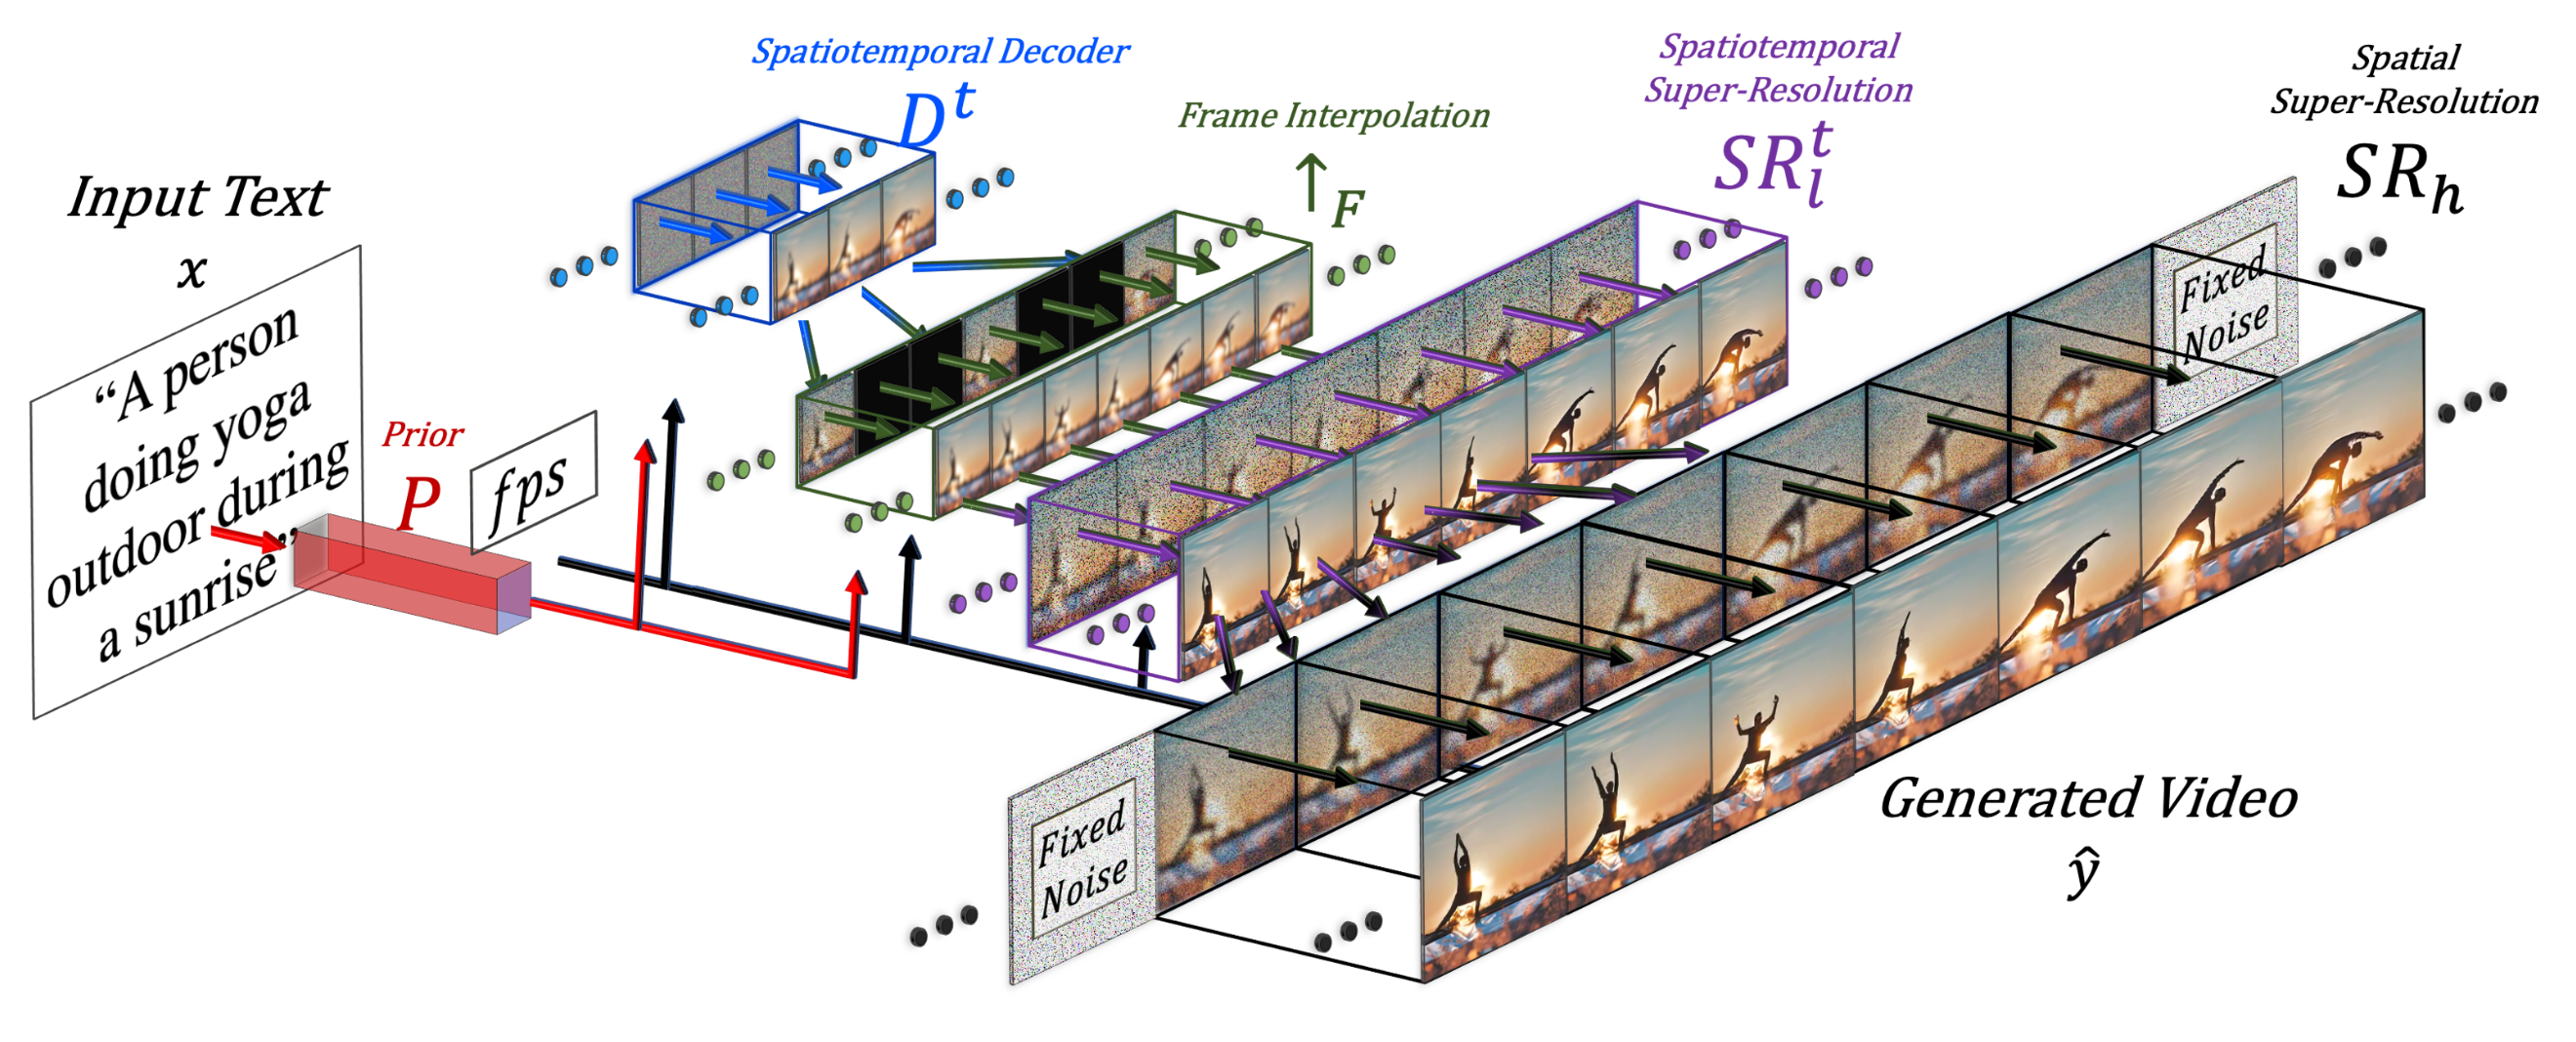
\includegraphics[width=1.0\textwidth]{images/emu_video_pipeline.png}
	\captionof{figure}{Sơ đồ quy trình hai bước của Emu Video. Một prompt văn bản đầu tiên được sử dụng để tạo ra một ảnh chất lượng cao. Sau đó, cả ảnh và prompt được đưa vào một mô hình video diffusion để tạo ra chuỗi video.}
	\label{fig:emu_video_pipeline}
\end{center}
% Keyword gợi ý: emu video architecture, factorized video generation

\subsection{Kling (Kuaishou, 2024): Video Dài và Chuyển động Phức tạp}
\label{subsec:kling_ai}
\textbf{Kling} là một mô hình T2V được phát triển bởi Kuaishou Technology (công ty mẹ của TikTok tại Trung Quốc), ra mắt vào giữa năm 2024. Nó đã gây ấn tượng mạnh với khả năng tạo ra các video dài tới 2 phút ở độ phân giải 1080p, với các chuyển động phức tạp và tuân thủ các quy luật vật lý.

\textbf{Đặc điểm Kỹ thuật Nổi bật:}
\begin{itemize}
	\item \textbf{Kiến trúc Diffusion Transformer (DiT):} Tương tự như Sora, Kling được cho là sử dụng một kiến trúc dựa trên Transformer để mô hình hóa các mối quan hệ không gian-thời gian, cho phép nó xử lý các phụ thuộc tầm xa hiệu quả.
	\item \textbf{Attention Không gian-Thời gian 3D:} Kling sử dụng một cơ chế attention 3D được tối ưu hóa, cho phép mô hình tập trung vào các vùng không gian và các khoảnh khắc thời gian một cách đồng thời, giúp tạo ra các chuyển động lớn và phức tạp (ví dụ: một người đang ăn mì, một con mèo đang lái xe).
	\item \textbf{Mô hình Thế giới Vật lý:} Khả năng tạo ra các video dài với các tương tác hợp lý cho thấy Kling, giống như Sora, đang học một mô hình nội tại về thế giới vật lý từ dữ liệu video khổng lồ.
\end{itemize}
Sự ra đời của Kling, ngay sau Sora, cho thấy một cuộc chạy đua toàn cầu trong việc xây dựng các mô hình sinh video quy mô lớn, và khẳng định vị thế của kiến trúc Diffusion Transformer như một hướng đi chủ đạo.

\subsection{Hướng tới Hợp nhất: Kết hợp Text, Video, và 3D}
\label{subsec:unified_multimodal_generation}
Tương lai của AI sáng tạo không nằm ở các mô hình đơn lẻ, mà ở các \textbf{pipeline (quy trình) đa phương thức} có khả năng chuyển đổi liền mạch giữa các loại dữ liệu khác nhau. Xu hướng 2024-2025 đang chứng kiến sự hội tụ của các lĩnh vực mà chúng ta đã thảo luận:
\begin{itemize}
	\item \textbf{Text $\rightarrow$ Video $\rightarrow$ 3D/4D Scene:} Một quy trình làm việc trong tương lai có thể bắt đầu bằng một prompt văn bản để tạo ra một video (sử dụng Sora hoặc Kling). Sau đó, một mô hình khác (dựa trên NeRF hoặc Gaussian Splatting) có thể nhận video đó làm đầu vào để tái tạo lại một cảnh 3D/4D động và tương tác được.
	\item \textbf{Video $\rightarrow$ 3D Reconstruction $\rightarrow$ Interactive Editing:} Người dùng có thể quay một đoạn video ngắn bằng điện thoại, hệ thống sẽ tự động tái tạo lại một mô hình 3D của đối tượng, và sau đó người dùng có thể chỉnh sửa mô hình 3D đó và tạo ra các video mới từ các góc nhìn khác nhau.
	\item \textbf{Tương tác Đa phương thức Toàn diện:} Các mô hình nền tảng như GPT-4o và Gemini đang mở đường cho một kỷ nguyên nơi người dùng có thể tương tác với AI bằng cách kết hợp văn bản, giọng nói, hình ảnh và video. Quá trình sáng tạo sẽ trở thành một cuộc "đối thoại" hai chiều, trong đó AI không chỉ nhận lệnh mà còn có thể đặt câu hỏi, yêu cầu làm rõ, và đề xuất các ý tưởng.
\end{itemize}

\subsection{Kết luận: Kỷ nguyên của các Cộng tác viên Sáng tạo}
\label{subsec:multimodal_gen_conclusion}
Các mô hình sinh đa phương thức như Emu và Kling đại diện cho một bước tiến hóa quan trọng của AI sáng tạo. Chúng không còn là những công cụ thụ động chỉ thực thi một lệnh, mà đang dần trở thành những cộng tác viên thông minh, có khả năng hiểu các ý tưởng phức hợp được diễn đạt qua nhiều kênh thông tin.

Bằng cách hợp nhất sức mạnh của các mô hình thị giác-ngôn ngữ, các mô hình khuếch tán không gian-thời gian, và các công nghệ kết xuất 3D, lĩnh vực này đang xây dựng nền tảng cho một tương lai của truyền thông tương tác, metaverse, và các công cụ sáng tạo thế hệ mới. Việc sản xuất nội dung số, từ các clip marketing đến các bộ phim bom tấn, có thể sẽ được định nghĩa lại hoàn toàn, giảm thiểu chi phí và rào cản kỹ thuật, và giải phóng sức sáng tạo không giới hạn của con người.

\section*{Tài liệu tham khảo}
\begin{itemize}
	\item[1] Dai, P., et al. (2023). Emu: Enhancing mascaraed autoencoders with multi-modal embeddings. \textit{arXiv preprint arXiv:2310.03713}. (Paper giới thiệu mô hình nền tảng Emu).
	\item[2] Girdhar, R., et al. (2023). Emu video: Factorizing text-to-video generation by explicit image synthesis. \textit{arXiv preprint arXiv:2311.10709}. (Paper giới thiệu Emu Video).
	\item[3] Kuaishou Technology. (2024). \textit{Kling Large Video Model Technical Report}. Kuaishou Technology Blog. (Công bố và các ví dụ về mô hình Kling).
	\item[4] OpenAI. (2024). \textit{Video generation models as world simulators}. OpenAI Technical Report. (Báo cáo kỹ thuật về Sora, cung cấp bối cảnh cho các mô hình T2V quy mô lớn).
	\item[5] Bar-Tal, O., et al. (2024). \textit{Lumiere: A Space-Time Diffusion Model for Video Generation}. Google Research. (Paper về Lumiere, một kiến trúc T2V quan trọng khác).
\end{itemize}